\textcolor{blue}{Problem 1}
In this problem, you will investigate the relationship between the soft order constraint and the augmented error. The regularized weight $\mathbf{w}_{\text {reg }}$ is a solution to
\begin{align*}
\min &\ E_{\text {in }}(\mathbf{w}) \\
\text {subject to} &\ \mathbf{w}^{\mathrm{T}} \Gamma^{\mathrm{T}} \Gamma \mathbf{w} \leq C
\end{align*}
(a) If $\mathbf{w}_{\text {lin }}^{\mathrm{T}} \Gamma^{\mathrm{T}} \Gamma \mathrm{w}_{\text {lin }} \leq C$, then what is $\mathbf{w}_{\text{reg}}$?\\
(b) If $\mathbf{w}_{\text {lin }}^\tau \Gamma^{\top} \Gamma \mathbf{w}_{\text {lin }}>C$, the situation is illustrated below,
\begin{figure}[htbp]
    \center
    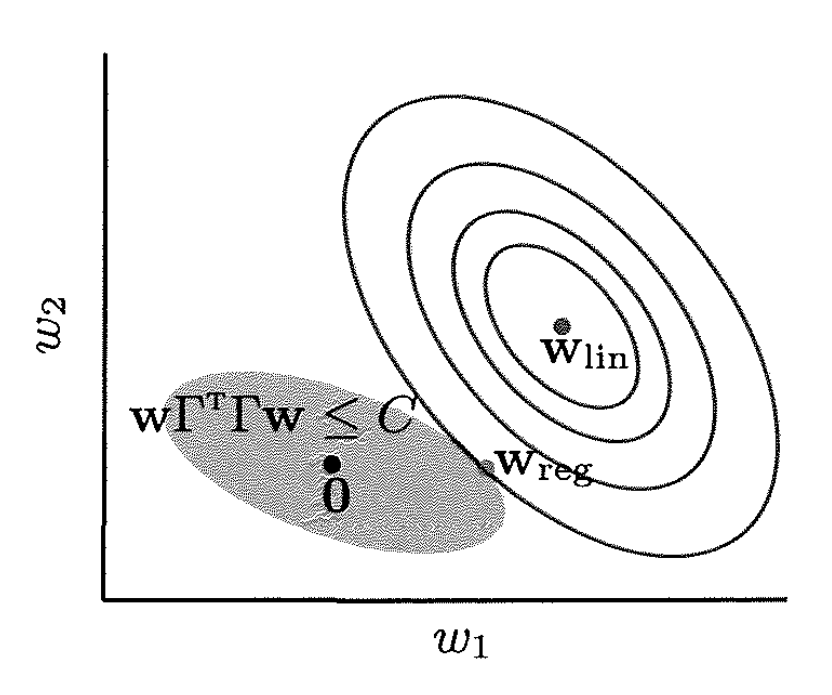
\includegraphics[width=0.5\textwidth]{../fig/p1.png}
\end{figure}

The constraint is satisfied in the shaded region and the contours of constant $E_{\text {in }}$ are the ellipsoids (why ellipsoids?). What is $\mathbf{w}_{\text {reg }}^{\mathrm{T}} \Gamma^{\mathrm{T}} \Gamma \mathbf{w}_{\mathrm{reg}}$?\\
(c) Show that with
$$
\lambda_C=-\frac{1}{2 C} \mathbf{w}_{\text {reg }}^{\mathrm{T}} \nabla E_{\text {in }}\left(\mathbf{w}_{\text {reg }}\right)
$$
$\mathbf{w}_{\text {reg }}$ minimizes $E_{\text {in }}(\mathbf{w})+\lambda_C \mathbf{w}^{\mathrm{T}} \Gamma^{\mathrm{T}} \Gamma \mathbf{w}$. [Hint: use the previous part to solve for $\mathbf{w}_{\text{reg}}$ as an equality constrained optimization problem using the method of Lagrange multipliers.]\\
(d) Show that the following hold for $\lambda_C$ :\\
(i) If $\mathrm{w}_{\text {lin }}^{\mathrm{T}} \Gamma^{T} \Gamma \mathbf{w}_{\text {lin }} \leq C$ then $\lambda_C=0$ ( $\mathbf{w}_{\text {lin }}$ itself satisfies the constraint).\\
(ii) If $\mathrm{w}_{\text {lin }}^{\mathrm{T}} \Gamma^{\mathrm{T}} \Gamma \mathrm{w}_{\text {lin }}>C$, then $\lambda_C>0$ (the penalty term is positive).\\
(iii) If $\mathrm{w}_{\text {lin }}^{\mathrm{T}} \Gamma^{\mathrm{T}} \Gamma \mathrm{w}_{\text {lin }}>C$, then $\lambda_C$ is a strictly decreasing function of $C$. [Hint: show that $\frac{d \lambda_C}{d C}<0$ for $\left.C \in\left[0, \mathbf{w}_{\text {lin }}^T \Gamma^T \Gamma \mathbf{w}_{\text {lin }}\right]\right]$.

\textcolor{blue}{Solution}\\
(a) Since $\mathbf{w}_{\text {lin }}^{\mathrm{T}} \Gamma^{\mathrm{T}} \Gamma \mathrm{w}_{\text {lin }} \leq C$, which has already suitable for the constrains, so $\mathbf{w}_{\text{reg}}=\mathbf{w}_{\text{lin}}$.\\
(b) 1. Firstly, we can prove that the contours of constant $E_{\text {in }}$ are the ellipsoids.\\
We can set $E_{\text {in }}(\mathbf{w})$ to be the $L_2$ loss, i.e.
$$E_{\text {in }}(\mathbf{w})=\frac{1}{N} \sum_{n=1}^{N}\left(\mathbf{w}^{\mathrm{T}} \mathbf{x}_{n}-y_{n}\right)^{2}=\dfrac{1}{N}\|\mathbf{Xw}-\mathbf{y}\|_2^2$$
where $\mathbf{X}$ is the matrix of feature vectors, $\mathbf{y}$ is the vector of labels, and $N$ is the number of data points, $\mathbf{x}_{n}$ is the feature vector of the $n$-th data point and $y_{n}$ is the label.

Consider the $\mathbf{w}$ in $2D$ dimensional case, where each feature vector has a dummy feature $x_2=1$, so $\mathbf{w}=\left[w_1,w_2\right]$, and $\mathbf{x}_n=\left[x_{n},1\right]$. Then the $E_{\text {in }}(\mathbf{w})$ can be written as
\begin{align*}
    E_{\text {in }}(\mathbf{w}) &= \dfrac{1}{N}\|\mathbf{Xw}-\mathbf{y}\|_2^2 \\
    &= \frac{1}{N} \sum_{n=1}^{N}\left(\mathbf{w}^{\mathrm{T}} \mathbf{x}_{n}-y_{n}\right)^{2} \\
    &= \frac{1}{N} \sum_{n=1}^{N}\left(w_1x_{n}+w_2-y_{n}\right)^{2} \\
    &= \frac{1}{N} \sum_{n=1}^{N}(w_1^2x_n^2+w_2^2+2w_1w_2x_n+C(w_1,w_2,x_n,y_n))
\end{align*}
Since we want to get the contours of constant $E_{\text {in }}$, so we just need to focus on the quadratic form of $E_{\text {in }}$, so $C(w_1,w_2,x_n,y_n)$ can be ignored.\\
Let $A=\dfrac{1}{N}\sum\limits_{n=1}^{N}x_n^2$, $B=\dfrac{1}{N}\sum\limits_{n=1}^{N}x_n$,$C=1$.\\
So 
$$E_{\text {in }}(\mathbf{w})=A\cdot w_1^2+2B\cdot w_1w_2+C\cdot w_2^2+\frac{1}{N} \sum_{n=1}^{N}C(w_1,w_2,x_n,y_n)$$
\begin{align*}
    AC-B^2 &= \dfrac{1}{N}\sum_{n=1}^{N}x_n^2\cdot 1-\left(\dfrac{1}{N}\sum_{n=1}^{N}x_n\right)^2 \\
    &= \dfrac{1}{N}\sum_{n=1}^{N}x_n^2-\dfrac{1}{N^2}\left(\sum_{n=1}^{N}x_n\right)^2 \\
    &= \dfrac{1}{N^2}\left[N\sum_{n=1}^{N}x_n^2-\left(\sum_{n=1}^{N}x_n\right)^2\right] \\
    &= \dfrac{1}{N^2}\left[(N-1)\sum_{n=1}^{N}x_n^2-\sum_{1\leq i<j\leq N}x_ix_j\right] \\
    &= \dfrac{1}{N^2}\left[\sum_{1\leq i<j\leq N}(x_i-x_j)^2\right] \\
    &\geq 0
\end{align*}

Since we can remove the duplicate data, i.e. make sure $x_i\neq x_j$, so $AC-B^2>0$, so the contours of constant $E_{\text {in }}$ are the ellipsoids.\\

2. Secondly, from the figure of contours, we can find that the minimum of $E_{\text {in }}$ which also fit the constraint is on the boundary of the constraint, i.e. the intersection of the objective function's contour and the constraint.\\
So we can find that
$$\mathbf{w}_{\text{reg}}^{\mathrm{T}} \Gamma^{\mathrm{T}} \Gamma \mathbf{w}_{\mathrm{reg}}=C$$

So above all, the contours of constant $E_{\text {in }}$ are the ellipsoids, and $\mathbf{w}_{\text{reg}}^{\mathrm{T}} \Gamma^{\mathrm{T}} \Gamma \mathbf{w}_{\mathrm{reg}}=C$.\\

(c) We can apply Lagrange multipliers to solve the problem.\\
The Lagrangian function is:
$$L(\mathbf{w},\lambda)=E_{\text {in }}(\mathbf{w})+\lambda (\mathbf{w}^{\mathrm{T}} \Gamma^{\mathrm{T}} \Gamma \mathbf{w}-C)$$
And its gradient is:
$$\nabla_{\mathbf{w}}L(\mathbf{w},\lambda)=\nabla E_{\text {in }}(\mathbf{w})+2\lambda\Gamma^{\mathrm{T}} \Gamma \mathbf{w}$$
To minimize $E_{\text {in }}(\mathbf{w})+\lambda \mathbf{w}^{\mathrm{T}} \Gamma^{\mathrm{T}} \Gamma \mathbf{w}$, we need to make sure that the gradient of $L(\mathbf{w},\lambda)$ is zero, so we have
\begin{align*}
    \nabla_{\mathbf{w}}L(\mathbf{w},\lambda)=0 &\Rightarrow \nabla E_{\text {in }}(\mathbf{w})+2\lambda\Gamma^{\mathrm{T}} \Gamma \mathbf{w}=0 \\
    &\Rightarrow 2\lambda\Gamma^{\mathrm{T}} \Gamma \mathbf{w}=-\nabla E_{\text {in }}(\mathbf{w}) \\
    &\Rightarrow 2\lambda\mathbf{w}^{\mathrm{T}} \Gamma^{\mathrm{T}} \Gamma \mathbf{w}=-\mathbf{w}^{\mathrm{T}} \nabla E_{\text {in }}(\mathbf{w}) \\ 
    &\Rightarrow \lambda=-\dfrac{1}{2\mathbf{w}^{\mathrm{T}} \Gamma^{\mathrm{T}} \Gamma \mathbf{w}}\mathbf{w}^{\mathrm{T}} \nabla E_{\text {in }}(\mathbf{w})
\end{align*}

1. If $\mathbf{w}_{\text{reg}}$ is a solution fits the primal feasibility, i.e. $\mathbf{w}_{\text{lin}}\Gamma^{T} \Gamma \mathbf{w}_{\text{lin}}\leq C$\\
Then we have
$$\mathbf{w}_{\text{reg}}=\mathbf{w}_{\text{lin}}$$
Since its the primal optimal points, so we also have
$$\nabla E_{\text {in }}(\mathbf{w}_{\text{reg}})=\nabla E_{\text {in }}(\mathbf{w}_{\text{lin}}) = 0$$
Then we also have
$$\lambda = 0$$


2. If $\mathbf{w}_{\text{lin}}\Gamma^{T} \Gamma \mathbf{w}_{\text{lin}}> C$, then we have
$$\mathbf{w}_{\text{reg}}\Gamma^{T} \Gamma \mathbf{w}_{\text{reg}}= C$$
So we have
$$\lambda = -\dfrac{1}{2C}\mathbf{w}_{\text{reg}}^T\nabla E_{\text{in}}(\mathbf{w}_{\text{reg}})$$

So combine the above two situations, we can get that with
$$\lambda = -\dfrac{1}{2C}\mathbf{w}_{\text{reg}}^T\nabla E_{\text{in}}(\mathbf{w}_{\text{reg}})$$
$\mathbf{w}_{\text{reg}}$ minimizes $E_{\text{in}}(\mathbf{w})+\lambda \mathbf{w}^{\mathrm{T}} \Gamma^{\mathrm{T}} \Gamma \mathbf{w}$.\\

(d) The KKT conditions of the optimization problem are:
\begin{equation}
\left\{\begin{array}{l}
    \mathbf{w}^T\Gamma^{T} \Gamma \mathbf{w}\leq C              \text{\ \ \ \ \ \ \ \ \ \ \ \ \ \ \ \ \ \ (primal feasibility)}\\
    \lambda\geq 0                                               \text{\ \ \ \ \ \ \ \ \ \ \ \ \ \ \ \ \ \ \ \ \ \ \ \ \ \ \ \ \ \ \ \ \ \ (dual feasibility)}\\
    \lambda(\mathbf{w}^T\Gamma^{T} \Gamma \mathbf{w}- C)=0      \text{\ \ \ \ \ \ (complementary slackness)}\\
    \nabla_{\mathbf{w}} L(\mathbf{w},\lambda)=0                  \text{\ \ \ \ \ \ \ \ \ \ \ \ \ \ \ \ \ (zero gradient of Lagrangian of $\mathbf{w}$)}
    \end{array}\right.
\label{KKT}
\end{equation}

(i) From the complementary slackness, we have 
$$\lambda(\mathbf{w}^T\Gamma^{T} \Gamma \mathbf{w}- C)=0$$
so if $\mathbf{w}_{\text{lin}}^T\Gamma^{T} \Gamma \mathbf{w}_{\text{lin}}\leq C$, i.e. $\mathbf{w}_{\text{weg}}=\mathbf{w}_{\text{lin}}$, we have
$$\mathbf{w}_{\text{weg}}^T\Gamma^{T} \Gamma \mathbf{w}_{\text{weg}} - C \neq 0$$
then $\lambda=0$.\\
From (c)'s 1. , we can also verify that $\lambda_C=0$.\\

(ii) From the dual feasibility, we have $$\lambda\geq 0$$
And if $\mathbf{w}_{\text{lin}}^T\Gamma^{T} \Gamma \mathbf{w}_{\text{lin}}>C$, 
From (c)'s 2. , we can also get that 
$$\lambda_C=-\dfrac{1}{2C}\mathbf{w}_{\text{reg}}^T\nabla E_{\text{in}}(\mathbf{w}_{\text{reg}})$$
We can use contradiction to prove that $\lambda>0$:\\
Suppose $\lambda_C=0$, then form KKT condition's zero gradient of Lagrangian of $\mathbf{w}$, we can get that
$$\nabla_{\mathbf{w}}L(\mathbf{w},\lambda)=\nabla E_{\text {in }}(\mathbf{w})+2\lambda\Gamma^{\mathrm{T}} \Gamma \mathbf{w} = 0$$
Since $\lambda_C=0$, so we can get that
$$\nabla E_{\text {in }}(\mathbf{w})=0$$
i.e. $\mathbf{w}_{\text{reg}}=\mathbf{w}_{\text{lin}}$.\\
However, we have known that $\mathbf{w}_{\text{lin}}^T\Gamma^{T} \Gamma \mathbf{w}_{\text{lin}}>C$, so its impossible.\\
So it contradicts.\\
i.e. it is not possible that $\lambda_C=0$.

So above all, we have proved that $\lambda_C>0$.\\

(iii) From (ii), we have get that
$$\lambda_C = -\frac{1}{2C}\mathbf{w}_{\text{reg}}^T\nabla E_{\text{in}}(\mathbf{w}_{\text{reg}})>0$$
When $C\to 0$, we can get that:
$C\to 0\Leftrightarrow\mathbf{w}\to \mathbf{0}$.\\
Since $C=\mathbf{w}^T\Gamma^{T}\Gamma\mathbf{w}=o(\|\mathbf{w}\|^2)$, and 
$$E_\text{in}(\mathbf{w})=\frac{1}{N}\|\mathbf{Xw}-\mathbf{y}\|_2^2$$
$$w^T\nabla E_{\text{in}}(\mathbf{w})=w^T\frac{2}{N}\mathbf{X}^T(\mathbf{Xw}-\mathbf{y})=o(\|\mathbf{w}\|^2+\|\mathbf{w}\|)=o(\|\mathbf{w}\|)$$
So
$$\lim_{C\to 0}\lambda_C=\lim_{\mathbf{w}\to \mathbf{0}}\dfrac{o(\|\mathbf{w}\|)}{o(\|\mathbf{w}\|^2)}=+\infty$$

And when $C>0$, we have:
$$\frac{d\lambda_C}{dC} = \frac{1}{2C^2}\mathbf{w}_{\text{reg}}^T\nabla E_{\text{in}}(\mathbf{w}_{\text{reg}})=-\dfrac{1}{C}\lambda_C < 0$$

So above all, $\lambda_C$ is a strictly decreasing function for $C \in\left[0, \mathbf{w}_{\text {lin }}^T \Gamma^T \Gamma \mathbf{w}_{\text {lin }}\right]$.

\newpage